\documentclass[9pt,aspectratio=169,xcolor=table]{beamer}

%~~~~~~~~~~~~~~~~~~~~~~~~~~~~~~~~~~~~~~~~~~~~~~~~~~~~~~~~~~~~~~~~~~~~~~~~~~~~~~
% Use roboto Font (recommended)
\usepackage[sfdefault]{roboto}
\usepackage[utf8]{inputenc}
\usepackage[T1]{fontenc}
%~~~~~~~~~~~~~~~~~~~~~~~~~~~~~~~~~~~~~~~~~~~~~~~~~~~~~~~~~~~~~~~~~~~~~~~~~~~~~~

%~~~~~~~~~~~~~~~~~~~~~~~~~~~~~~~~~~~~~~~~~~~~~~~~~~~~~~~~~~~~~~~~~~~~~~~~~~~~~~
% Define where theme files are located. ('/styles')
\usepackage{styles/fluxmacros}
\usefolder{styles}
% Use Flux theme v0.1 beta
% Available style: asphalt, blue, red, green, gray
\usetheme[style=gray]{flux}
%~~~~~~~~~~~~~~~~~~~~~~~~~~~~~~~~~~~~~~~~~~~~~~~~~~~~~~~~~~~~~~~~~~~~~~~~~~~~~~

%~~~~~~~~~~~~~~~~~~~~~~~~~~~~~~~~~~~~~~~~~~~~~~~~~~~~~~~~~~~~~~~~~~~~~~~~~~~~~~
% Extra packages
\usepackage{booktabs}
\usepackage{colortbl}
\usepackage{ragged2e}
\usepackage{amssymb}
\usepackage{multirow}
\usepackage{tikz}
\usetikzlibrary{arrows.meta, positioning, fit, backgrounds, calc, decorations.pathreplacing}
\setbeamertemplate{itemize items}[square]
\usepackage[scaled=.92]{beramono}
\usepackage{listings}
\usepackage{styles/lstlangarm}
\usepackage{array}
\definecolor{bgcolor}{HTML}{F2E9E9}
% lstlangarm.sty references \color{mauve} for string literals but never defines
% it -- only fires when a listing contains a string. Define it here.
\definecolor{mauve}{rgb}{0.58,0,0.82}
% lstlangarm's C style sets commentstyle=green!20, which is unreadable on the
% pink listing background. Darken it globally.
\lstset{commentstyle=\color{green!45!black}}
% ragged-right fixed-width column -- must be defined in the preamble, never
% inside a frame (\newcolumntype's #1 breaks beamer's frame scanner)
\newcolumntype{R}[1]{>{\RaggedRight\arraybackslash}p{#1}}
%~~~~~~~~~~~~~~~~~~~~~~~~~~~~~~~~~~~~~~~~~~~~~~~~~~~~~~~~~~~~~~~~~~~~~~~~~~~~~~
% Table striping: odd rows white, even rows very light gray.
% Needs \documentclass[...,xcolor=table]{beamer} (beamer loads xcolor itself,
% so the option must go on the class, not \usepackage).
\definecolor{stripe}{gray}{0.94}
% \striped makes body rows alternate white, gray, white, ... starting white.
% \rowcolors counts from the first coloured body row; the header is not counted.
\newcommand{\striped}{\rowcolors{1}{white}{stripe}}
%~~~~~~~~~~~~~~~~~~~~~~~~~~~~~~~~~~~~~~~~~~~~~~~~~~~~~~~~~~~~~~~~~~~~~~~~~~~~~~

%~~~~~~~~~~~~~~~~~~~~~~~~~~~~~~~~~~~~~~~~~~~~~~~~~~~~~~~~~~~~~~~~~~~~~~~~~~~~~~
% TikZ block styles -- matches ch1/ch2
% Colour variables are named identically in the book's stm32primer.tex, so any
% tikzpicture using only the \tikzset{...} styles below can be copied verbatim
% between slides and book. Only the \definecolor/\colorlet VALUES differ: the
% book is printed, so it keeps every stroke pure black with muted fills. These
% slides are projected, so both fill AND stroke are bright and saturated to
% grab attention -- see stm32primer.tex for the print palette.
\definecolor{blkfill}{HTML}{DCEBFF}
\definecolor{blkline}{HTML}{1565C0}
\definecolor{accentfill}{HTML}{FFE0B2}
\definecolor{accentline}{HTML}{E65100}
\definecolor{memfill}{HTML}{DFF5DA}
\definecolor{memline}{HTML}{2E7D32}
\definecolor{cellfill}{HTML}{FFFFFF}
\definecolor{cellline}{HTML}{424242}
\definecolor{bitmaskfill}{HTML}{DCEBFF}
\definecolor{bitmaskline}{HTML}{1565C0}
\definecolor{bithitfill}{HTML}{FFE0B2}
\definecolor{bithitline}{HTML}{E65100}
\tikzset{
  blk/.style   = {rectangle, rounded corners=2pt, draw=blkline, fill=blkfill,
                  thick, align=center, font=\small, minimum height=9mm, inner sep=3pt},
  cpublk/.style= {rectangle, rounded corners=2pt, draw=accentline, fill=accentfill,
                  thick, align=center, font=\small\bfseries, minimum height=9mm, inner sep=3pt},
  memblk/.style= {rectangle, rounded corners=2pt, draw=memline, fill=memfill,
                  thick, align=center, font=\small, minimum height=9mm, inner sep=3pt},
  cell/.style  = {rectangle, draw=cellline, fill=cellfill, align=center,
                  font=\normalsize\ttfamily, minimum height=7mm, inner sep=2pt},
  lbl/.style   = {font=\scriptsize, text=Gray},
  flow/.style  = {-{Stealth[length=2mm]}, thick, draw=blkline},
  busline/.style={thick, draw=cellline},
}
% NOTE (theme quirks -- all fail SILENTLY, always page through the PDF):
%  - a second \\ inside a nested {...} group in a TikZ node breaks parsing
%  - {\small ...} wrapped around a nested itemize eats the frame title + list
%  - \usebeamercolor on a [plain] frame falls through to an unstyled default
%  - \newcolumntype inside a frame breaks beamer's frame scanner
%  - lstlisting needs \begin{frame}[fragile]
%  - a TikZ picture wider than its column silently overflows into neighbours
%~~~~~~~~~~~~~~~~~~~~~~~~~~~~~~~~~~~~~~~~~~~~~~~~~~~~~~~~~~~~~~~~~~~~~~~~~~~~~~

%%%%%%%%%%%%%%%%%%%%%%%%%%%%%%%%%%%
%% BEGIN CONDITIONAL COMPILATION %%
%%%%%%%%%%%%%%%%%%%%%%%%%%%%%%%%%%%
\newif\ifwebex
%\webextrue % uncomment to generate section separator
\ifwebex
\AtBeginSection[]{
  \begin{frame}
  \vfill
  \centering
  \begin{beamercolorbox}[sep=8pt,center,shadow=true,rounded=true]{title}
    \usebeamerfont{title}\insertsectionhead\par%
  \end{beamercolorbox}
  \vfill
  \end{frame}
}
\else
\AtBeginSection[]
{
{
    \setbeamercolor{background canvas}{bg=yellow!10}
    \begin{frame}[plain]
        \frametitle{Table of Contents}
        \tableofcontents[currentsection]
    \end{frame}
}
}
\fi
%%%%%%%%%%%%%%%%%%%%%%%%%%%%%%%%%%%
%% END CONDITIONAL COMPILATION   %%
%%%%%%%%%%%%%%%%%%%%%%%%%%%%%%%%%%%

%~~~~~~~~~~~~~~~~~~~~~~~~~~~~~~~~~~~~~~~~~~~~~~~~~~~~~~~~~~~~~~~~~~~~~~~~~~~~~~
% Information
\title{Control Flow, Functions and the Stack}
\subtitle{\emph{Introduction to ARM Cortex-M Microprocessors} --- Chapter 7}
\author{Mun\'{i}m Zabidi}
\institute{\color{primary}Faculty of Electrical Engineering, Universiti Teknologi Malaysia}
\date{\today}
\titlegraphic{assets/logoutmwhite.png}
%~~~~~~~~~~~~~~~~~~~~~~~~~~~~~~~~~~~~~~~~~~~~~~~~~~~~~~~~~~~~~~~~~~~~~~~~~~~~~~

\begin{document}

\titlepage

\begin{frame}{Table of Contents}
    \tableofcontents
\end{frame}

%===============================================================================
\section{Why This Matters}
%===============================================================================

\begin{frame}{Why This Chapter Matters}
    \leavevmode
    Every \texttt{if}, every \texttt{while}, and every function call you write in C becomes the same thing on the processor: a comparison that sets flags, and a branch that tests them. Understanding this mechanism explains things that seem mysterious. Why can an unsigned comparison give a different answer than a signed one, on the exact same bits? Why can a recursive function crash a microcontroller? Why does a function that forgets one instruction never return? This chapter also prepares you for interrupts. An interrupt is a function call that the hardware makes on its own.
\end{frame}

\begin{frame}{Objectives}
    \leavevmode
    {\small After completing this chapter, you should be able to:}

    \vspace{2mm}
    {\small
    \begin{enumerate}\itemsep2pt
        \item Explain the effect of the \texttt{S} suffix on the APSR flags, and use condition codes for conditional execution.
        \item Use \texttt{CMP}, \texttt{TST}, and the condition-code suffixes to branch on a computed condition.
        \item Tell signed and unsigned comparison suffixes apart, and choose the correct one for a given kind of data.
        \item Translate C \texttt{if}/\texttt{else} statements and loops into equivalent assembly.
        \item Explain how a full descending stack works, and trace SP through \texttt{PUSH} and \texttt{POP}.
        \item Call and return from subroutines using \texttt{BL} and \texttt{BX LR}, and explain why nested calls must preserve LR.
        \item State the AAPCS rules for argument passing, return values, and which registers a function must preserve.
    \end{enumerate}}
\end{frame}


%===============================================================================
\section{Flags and Conditions}
%===============================================================================

\begin{frame}{Processor Status Register}
    \centering
    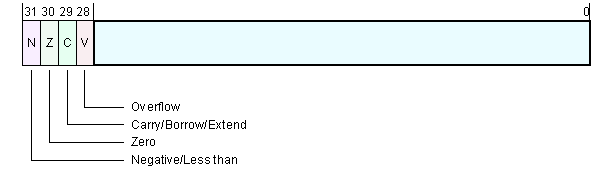
\includegraphics{assets/program_status_register.pdf}
    \vfill
    \renewcommand\arraystretch{1.2}\striped
    \begin{tabular}{c p{.6\textwidth}}
        \toprule
        \textbf{Flag} & \textbf{Description} \\
        \midrule
        N & 1 means result is negative \\
        Z & 1 means result is zero \\
        C & unsigned add: 1 means result had a carry out; unsigned subtract: 0 means it had a borrow; shifts: the bit shifted out \\
        V & signed add/subtract: 1 means the result overflowed \\
        \bottomrule
    \end{tabular}
\end{frame}

\begin{frame}[fragile]{Setting the Flags}
    \begin{columns}[T]
    \begin{column}{.46\textwidth}
        \textbf{The \texttt{S} suffix}

        \vspace{1mm}
        \begin{lstlisting}[style=armasm, basicstyle=\footnotesize\ttfamily]
ADD  R0, R1, R2   ; flags unchanged

ADDS R0, R1, R2   ; updates N Z C V
        \end{lstlisting}
    \end{column}
    \begin{column}{.5\textwidth}
        \textbf{Compare and test --- no result kept}

        \vspace{1mm}
        {\small
        \striped
        \begin{tabular}{@{}l l@{}}
            \toprule
            \textbf{Instruction} & \textbf{Computes} \\
            \midrule
            \texttt{CMP Rn, Op2} & \texttt{Rn $-$ Op2} \\
            \texttt{CMN Rn, Op2} & \texttt{Rn $+$ Op2} \\
            \texttt{TST Rn, Op2} & \texttt{Rn \& Op2} \\
            \texttt{TEQ Rn, Op2} & \texttt{Rn \^{} Op2} \\
            \bottomrule
        \end{tabular}}
    \end{column}
    \end{columns}

    \vspace{3mm}
    \begin{block}{Why compilers care about \texttt{S}}
        A compiler writes \texttt{SUBS} instead of \texttt{SUB} when a
        branch right after it needs the flags. So seeing \texttt{S} in a
        listing tells you \alert{a decision is coming}.
    \end{block}

    \vspace{1mm}
    {\small \texttt{CMP} is \texttt{SUBS} that throws the answer away.}
\end{frame}

\begin{frame}{Condition Codes}
    \begin{columns}[T]
    \begin{column}{.48\textwidth}
    	\centering
        {\normalsize
        \striped
        \begin{tabular}{@{}l l l@{}}
            \toprule
            \textbf{Code} & \textbf{Meaning} & \textbf{Flags} \\
            \midrule
            \texttt{EQ} & Equal            & \texttt{Z=1} \\
            \texttt{NE} & Not equal        & \texttt{Z=0} \\
            \texttt{MI} & Negative         & \texttt{N=1} \\
            \texttt{PL} & Positive or zero & \texttt{N=0} \\
            \texttt{VS} & Overflow         & \texttt{V=1} \\
            \texttt{AL} & Always (default) & --- \\
            \bottomrule
        \end{tabular}}
    \end{column}
    \begin{column}{.48\textwidth}
    	\centering
        {\normalsize
        \striped
        \begin{tabular}{@{}l l l@{}}
            \toprule
            \textbf{Code} & \textbf{Meaning} & \textbf{Flags} \\
            \midrule
            \texttt{HS/CS} & Unsigned $\geq$ & \texttt{C=1} \\
            \texttt{LO/CC} & Unsigned $<$    & \texttt{C=0} \\
            \texttt{HI}    & Unsigned $>$    & \texttt{C=1, Z=0} \\
            \texttt{LS}    & Unsigned $\leq$ & \texttt{C=0 or Z=1} \\
            \midrule
            \texttt{GE}    & Signed $\geq$   & \texttt{N=V} \\
            \texttt{LT}    & Signed $<$      & \texttt{N$\neq$V} \\
            \texttt{GT}    & Signed $>$      & \texttt{Z=0, N=V} \\
            \texttt{LE}    & Signed $\leq$   & \texttt{Z=1 or N$\neq$V} \\
            \bottomrule
        \end{tabular}}
    \end{column}
    \end{columns}

    \vspace{2mm}
    \begin{block}{Signed and unsigned comparisons are different instructions}
        \texttt{GT} and \texttt{HI} both mean ``greater than.'' But one
        reads \texttt{N} and \texttt{V}, and the other reads \texttt{C}
        and \texttt{Z}. \alert{Use a signed code for signed data}: for
        example, $-1 > 5$ is false when signed, but true when unsigned.
    \end{block}
\end{frame}

%===============================================================================
\section{Branches and Control Structures}
%===============================================================================

\begin{frame}{Branch Instructions}
    A branch writes a new value into the Program Counter. This redirects execution. Four forms matter:

    \vspace{2mm}
    \begin{center}
    {\normalsize
    \striped
    \begin{tabular}{@{}l l@{}}
        \toprule
        \textbf{Instruction} & \textbf{Meaning} \\
        \midrule
        \texttt{B label}   & Unconditional branch --- the basic jump \\
        \texttt{BL label}  & \emph{Branch with link} --- LR = return address, then jump: a subroutine call \\
        \texttt{BX Rn}     & \emph{Branch and exchange} to an address in a register; \texttt{BX LR} returns \\
        \texttt{BLX Rn}    & Call a subroutine whose address is in a register (function pointers) \\
        \bottomrule
    \end{tabular}}
    \end{center}

    \vspace{3mm}
    \begin{block}{Function addresses have their low bit set}
        The Cortex-M4 executes only Thumb instructions. \alert{Function
        addresses therefore have bit~0 set} to mark a valid Thumb
        target, and \texttt{BX}/\texttt{BLX} check it. In a debugger,
        this looks like an off-by-one error, until you know to expect
        it.
    \end{block}
\end{frame}

\begin{frame}{All Control Structures Are Just Branches}
    \leavevmode
    {\small Every high-level control structure you are about to see is built
    from exactly the two pieces just introduced: a \alert{comparison that sets
    flags}, and a \alert{conditional branch} that tests them. Nothing new is
    added --- only combined.}

    \vspace{3mm}
    \begin{center}
    {\small
    \striped
    \begin{tabular}{@{}l l@{}}
        \toprule
        \textbf{C construct} & \textbf{Built from} \\
        \midrule
        \texttt{if}        & one conditional branch \\
        \texttt{if}/\texttt{else} & one conditional branch \textbf{+} one unconditional branch \\
        \texttt{while}     & one conditional branch \textbf{+} one backward branch \\
        \texttt{do}/\texttt{while} & one backward conditional branch, no forward branch at all \\
        \bottomrule
    \end{tabular}}
    \end{center}

    \vspace{3mm}
    {\small Keep this map in view through the next few slides: each worked
    example below is one more arrangement of the same two pieces, never a new
    mechanism.}
\end{frame}

\begin{frame}{The \texttt{if} Construct}
    \begin{columns}[T]
    \begin{column}{.26\textwidth}
        \centering
        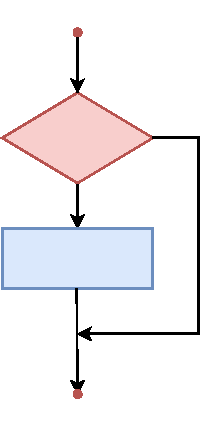
\includegraphics[width=.85\textwidth]{assets/struct-if.pdf}
    \end{column}
    \begin{column}{.72\textwidth}
        \centering
        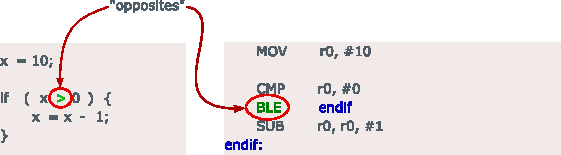
\includegraphics[width=.95\textwidth]{assets/opposites.pdf}

        \vspace{4mm}
        {\small\alert{Read the branch as the opposite of the C
        condition}: the code tests \texttt{x > 0}. The assembly
        branches away with \texttt{BLE} to \emph{skip} the body when
        this is not true.}
    \end{column}
    \end{columns}
\end{frame}

\begin{frame}[fragile]{The \texttt{if-else} Construct}
    \begin{columns}[T]
    \begin{column}{.22\textwidth}
        \centering
        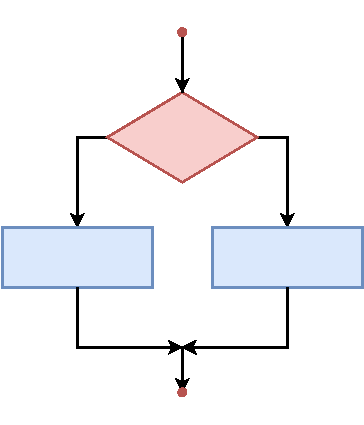
\includegraphics[width=.85\textwidth]{assets/struct-if-else.pdf}
    \end{column}
    \begin{column}{.34\textwidth}
        \begin{lstlisting}[style=myc, basicstyle=\footnotesize\ttfamily]
if (a == b)
    x = 1;
else
    x = 2;
        \end{lstlisting}
    \end{column}
    \begin{column}{.4\textwidth}
        \begin{lstlisting}[style=armasm, basicstyle=\footnotesize\ttfamily]
P   R0, R1          ; Compare a (R0) and b (R1)
        BNE   else_block      ; If Z == 0 (not equal), branch to else

        ; If-block: a == b
        MOV   R2, #1          ; x = 1
        B     endif           ; Branch past the else block

else_block
        ; Else-block: a != b
        MOV   R2, #2          ; x = 2

endif
    \end{lstlisting}
    \end{column}
    \end{columns}

    \vspace{3mm}
    \begin{block}{Both arms fall through without \texttt{B endif}}
        The \texttt{true} arm must jump past the \texttt{else} arm.
        Without \texttt{B endif}, execution falls through and runs
        both arms.
    \end{block}
\end{frame}

\begin{frame}[plain]{The Two Paths Through an \texttt{if-else}}
    \leavevmode
    \begin{center}
    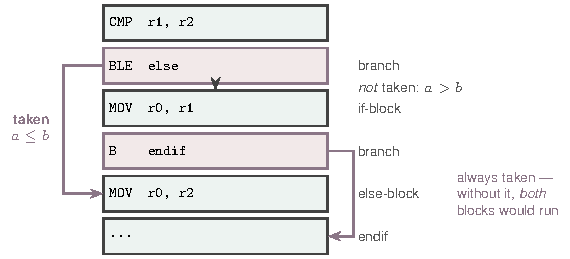
\includegraphics[width=.66\textwidth]{assets/ifelse-flow.pdf}
    \end{center}

    \vspace{1mm}
    {\small\centering The conditional branch tests the \emph{opposite}
    condition and jumps over the if-block; the unconditional branch
    jumps over the else-block. Execution reaches exactly one
    \texttt{MOV} --- never zero, never both.\par}
\end{frame}

\begin{frame}[fragile]{The \texttt{while} Construct}
    \begin{itemize}
        \item Implements both the \alert{while} and \alert{for} keywords in C
        \item The condition is tested \alert{before} the loop starts: a pre-test loop
    \end{itemize}
    \begin{center}
        \textbf{\texttt{sum = 1+2+3+4+5}}
    \end{center}
\vspace{1mm}
    \begin{columns}[T]
    \begin{column}{.22\textwidth}
        \centering
        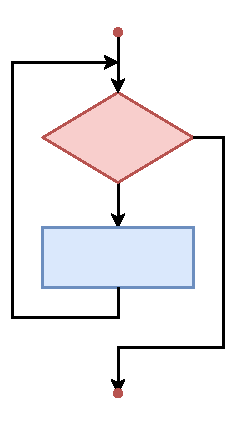
\includegraphics[scale=.55]{assets/struct-while.pdf}
    \end{column}
    \begin{column}{.37\textwidth}
        \begin{lstlisting}[style=myc, basicstyle=\footnotesize\ttfamily]
sum = 0;
for (i = 1; i <= 5; i++)
    sum = sum + i;
        \end{lstlisting}
    \end{column}
    \begin{column}{.37\textwidth}
        \begin{lstlisting}[style=armasm, basicstyle=\footnotesize\ttfamily]
		MOV   r0, #0
		MOV   r1, #1
loop
 	   CMP   r0, #5
 	   BGT   done
 	   ADD   r0, r0, r1
 	   ADD   r1, r1, #1
 	   B     loop
done
        \end{lstlisting}
    \end{column}
    \end{columns}
\end{frame}

\begin{frame}[fragile]{Worked Example: Popcount}
    \begin{itemize}
        \item \textbf{Popcount} (population count) means counting the number of bits that are 1
    \end{itemize}

    \vspace{1mm}
    {\small This example is primarily about \alert{reusing flags generated by
    another instruction}: \texttt{LSRS} shifts \emph{and} sets flags, so one
    instruction does the work \texttt{while} needed anyway.}

    \vspace{2mm}
    \begin{columns}[T]
    \begin{column}{.46\textwidth}
        \begin{lstlisting}[style=myc]
int x = 0x5555;   // input
int c = 0;
for (; x != 0; x >>= 1)
    if (x & 1)
        c++;
        \end{lstlisting}
    \end{column}
    \begin{column}{.5\textwidth}
        \begin{lstlisting}[style=armasm]
		LDR   r1, =0x5555
		MOV   r0, #0       ; count = 0
loop
		AND   r2, r1, #1   ; check bit 0
		ADD   r0, r2       ; c++
    	LSRS  r1, r1, #1   ; next bit
    	BNE   loop
done
        \end{lstlisting}
    \end{column}
    \end{columns}

    \vspace{3mm}
    \begin{block}{A new principle: one instruction, two jobs}
        \alert{\texttt{LSRS}} shifts \emph{and} sets \textbf{Z} when the
        remaining bits reach zero, so the shift itself supplies the
        condition the next branch needs --- no separate comparison.
        This is the same \texttt{S}-suffix idea from two slides ago,
        now doing useful work \emph{and} preparing the next decision.
        Note: if \texttt{x} starts at 0, this loop still runs once.
    \end{block}
\end{frame}

\begin{frame}[fragile]{The \texttt{do-while} Construct}
    \leavevmode
    {\small The condition is tested \alert{after} the loop body runs: a post-test loop.}
    \begin{center}
	\textbf{\texttt{sum = 1+2+3+4+5}}
	\end{center}
    \vspace{1mm}
    \begin{columns}[T]
    \begin{column}{.2\textwidth}
        \centering
        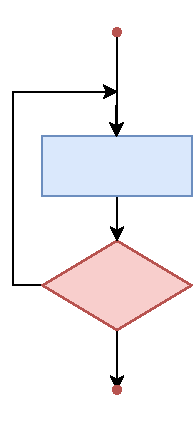
\includegraphics[width=.85\textwidth]{assets/struct-do-while.pdf}
    \end{column}
    \begin{column}{.37\textwidth}
        \begin{lstlisting}[style=myc, basicstyle=\footnotesize\ttfamily]
sum = 0;
i = 1;
do {
    sum = sum + i;
    i++;
} while (i <= 5);
        \end{lstlisting}
    \end{column}
    \begin{column}{.4\textwidth}
        \begin{lstlisting}[style=armasm, basicstyle=\footnotesize\ttfamily]
		MOV   r0, #0
		MOV   r1, #1
loop
    	ADD   r0, r0, r1
    	ADD   r1, r1, #1
    	CMP   r1, #5
    	BLE   loop
    \end{lstlisting}
    \end{column}
    \end{columns}

    \vspace{1mm}
    {\small A \texttt{do-while} always runs its body at least once. The
    comparison comes after the work, not before.}
\end{frame}

\begin{frame}[fragile]{Loops: Counting Down Is Cheaper}
    \leavevmode
    {\small The flags are not only for comparisons --- an arithmetic
    instruction with the \texttt{S} suffix can supply them too, exactly
    as \texttt{LSRS} did in \textbf{Popcount}.}

    \vspace{1mm}
    \begin{columns}[T]
    \begin{column}{.48\textwidth}
        \textbf{Counting up}

        \vspace{1mm}
        \begin{lstlisting}[style=armasm, basicstyle=\ttfamily\small]
     MOV  r0, #0
loop
     ...          ; body
     ADD  r0, #1
     CMP  r0, #10
     BLT  loop
        \end{lstlisting}

        \vspace{3mm}
        {\small \alert{Three} instructions of overhead per iteration.}
    \end{column}
    \begin{column}{.48\textwidth}
        \textbf{Counting down}

        \vspace{1mm}
        \begin{lstlisting}[style=armasm, basicstyle=\ttfamily\small]
     MOV  r0, #10
loop
     ...          ; body
     SUBS r0, #1  ; and set flags
     BNE  loop
        \end{lstlisting}

        \vspace{3mm}
        {\small \alert{Two} --- the \texttt{CMP} is gone.}
    \end{column}
    \end{columns}

    \vspace{2mm}
    \begin{block}{Why the \texttt{S} suffix saves an instruction}
        \texttt{SUBS} decrements \emph{and} sets \textbf{Z} when the
        result reaches zero, so no separate comparison is needed. This
        is the most common hand-optimisation in ARM assembly, and
        compilers do it automatically whenever the loop order does not
        matter.
    \end{block}
\end{frame}

\begin{frame}[fragile]{Worked Example: Find Maximum}
    \begin{itemize}
        \item Find the biggest signed word value in a memory block, starting at a known address
    \end{itemize}

    \vspace{1mm}
    \begin{columns}[T]
    \begin{column}{.4\textwidth}
        \begin{lstlisting}[style=myc]
int max = 0;
int *ptr = (int *)0x20001000;
int nwords = 64;
do {
    if (*ptr > max)
        max = *ptr;
    ptr++;
    nwords--;
} while (nwords);
        \end{lstlisting}
    \end{column}
    \begin{column}{.58\textwidth}
        \begin{lstlisting}[style=armasm]
		MOV    r0, #0          ; max
		LDR    r1, =0x20001000 ; ptr
		MOV    r2, #64         ; nwords
loop
    	LDR    r3, [r1], #4   ; *ptr, ptr++
    	CMP    r0, r3
    	BGE    skip
    	MOV    r0, r3         ; new max
skip	SUBS   r2, #1
    	BNE    loop
        \end{lstlisting}
    \end{column}
    \end{columns}

    \vspace{2mm}
    \begin{block}{\texttt{LDR Rn, =value} loads a number, not a variable}
        \texttt{ptr} and \texttt{nwords} hold a \emph{fixed} starting
        address and count, known at compile time. The assembly loads
        those known values directly into \texttt{r1}/\texttt{r2} ---
        there is no need to read \texttt{ptr}/\texttt{nwords} back out
        of memory, since nothing else in the program ever changes them.
    \end{block}
\end{frame}

%===============================================================================
\section{The Stack}
%===============================================================================

\begin{frame}{What Is a Stack?} \begin{itemize} \item A \alert{stack} is a region of ordinary SRAM managed using the \alert{Stack Pointer (SP, R13)}. \item It follows a \alert{last-in, first-out (LIFO)} rule: the most recently stored item is the first one removed. \item The stack can be located anywhere in the memory map. \item It is commonly used to hold \alert{return addresses}, \alert{saved registers}, and \alert{local variables}. \item All subroutines typically share the same stack. \end{itemize} \vspace{2mm} \begin{columns}[c] \begin{column}{.5\textwidth} \centering 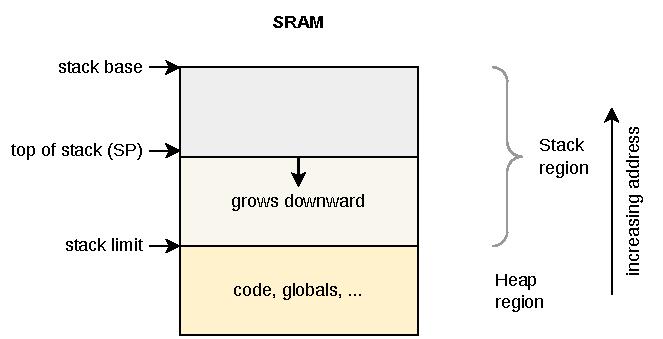
\includegraphics[width=.95\textwidth]{assets/what_is_a_stack.pdf} \end{column} \begin{column}{.46\textwidth} {\small \begin{itemize} \item The stack is typically initialized at the \alert{top of SRAM}. \item Initially, \texttt{SP} points to the top of the stack region. \item As items are pushed, \texttt{SP} moves toward \alert{lower addresses}. \item The heap, when present, typically grows upward from the opposite direction. \end{itemize} } \end{column} \end{columns} \end{frame}

%-------------------------------------------------------------------------------
\begin{frame}{How Does the Stack Grow?} \begin{itemize} \item The stack grows and shrinks by moving the \alert{Stack Pointer (SP)}. \item On a 32-bit Cortex-M processor, each stack word occupies \alert{4 bytes}. \end{itemize} \vspace{2mm} \begin{columns}[T] \begin{column}{.48\textwidth} \begin{block}{PUSH} \begin{enumerate} \item Move SP down by 4 bytes: \[ SP \leftarrow SP - 4 \] \item Store the value at the new SP address. \end{enumerate} \end{block} \end{column} \begin{column}{.48\textwidth} \begin{block}{POP} \begin{enumerate} \item Read the value at the current SP address. \item Move SP up by 4 bytes: \[ SP \leftarrow SP + 4 \] \end{enumerate} \end{block} \end{column} \end{columns} \vfill \centering 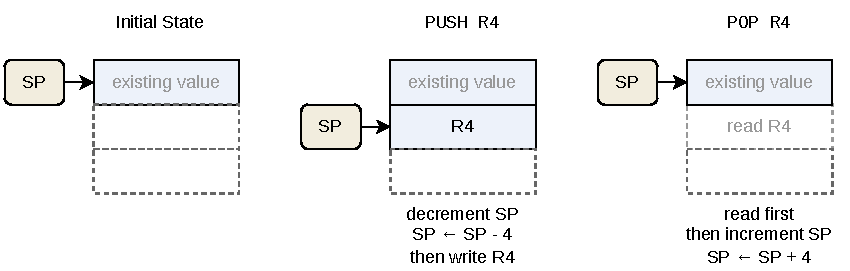
\includegraphics[width=.7\textwidth]{assets/push_pop.pdf} \end{frame}

%-------------------------------------------------------------------------------
\begin{frame}[plain]{Why Is It Called Last-In, First-Out?} \leavevmode \begin{center} 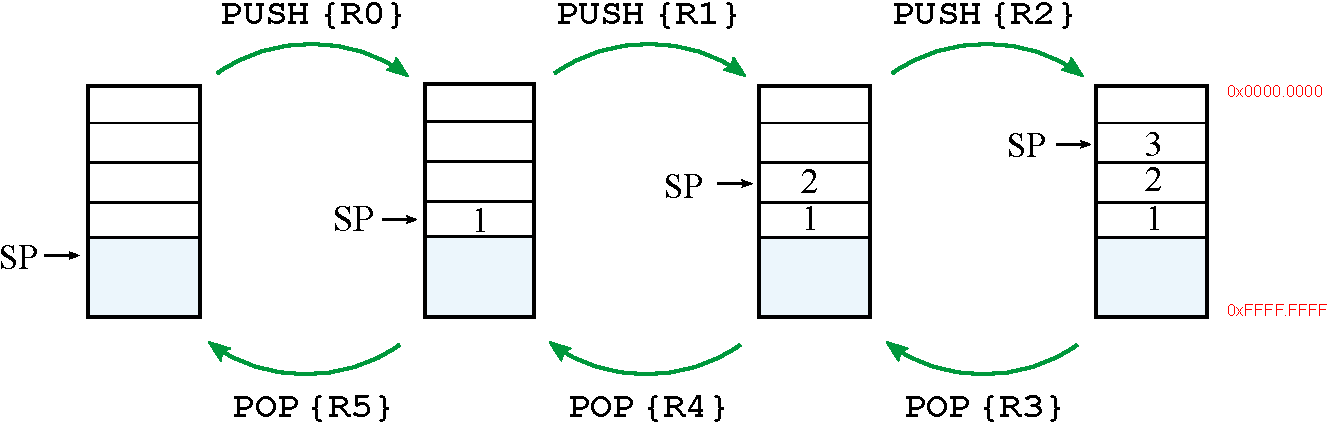
\includegraphics[width=.7\textwidth]{assets/push-pop-express.pdf} \end{center} \vspace{3mm} {\small Three \texttt{PUSH} operations place three registers on the stack. Because each new value is placed on top of the previous one, the first \texttt{POP} retrieves the value pushed last. } \vspace{2mm} \begin{block}{The LIFO rule} \centering The \alert{last value pushed} is the \alert{first value popped}. \end{block} \end{frame}

%-------------------------------------------------------------------------------
\begin{frame}{The Stack Must Stay Balanced} \begin{itemize} \item A subroutine may use the stack temporarily to save registers or other data. \item Before returning, it must restore the stack to the state it had on entry. \item In simple terms: \[ \boxed{\text{Every PUSH must eventually have a matching POP.}} \] \end{itemize} \vspace{3mm} \begin{block}{Example} \centering 3 registers pushed $\;\longrightarrow\;$ SP moves down by $3\times4=12$ bytes $\;\longrightarrow\;$ 3 registers popped $\;\longrightarrow\;$ SP returns to its original value \end{block} \vspace{3mm} {\small The order matters too: values must be popped in the \alert{reverse order} in which they were pushed. } \end{frame} %-------------------------------------------------------------------------------
\begin{frame}{What Happens When the Rules Are Broken?} \leavevmode {\small The stack is ordinary memory. If \texttt{SP} moves outside the space or contents intended for the stack, the program can behave unpredictably. } \vspace{3mm} \begin{columns}[T] \begin{column}{.48\textwidth} \begin{block}{Too many PUSHes} \begin{itemize}\itemsep2pt \item \texttt{SP} keeps moving toward lower addresses. \item The stack can exceed its allocated region. \item It may collide with other memory regions. \item This is commonly called \alert{stack overflow}. \end{itemize} \end{block} \end{column} \begin{column}{.48\textwidth} \begin{block}{Too many POPs} \begin{itemize}\itemsep2pt \item \texttt{SP} moves beyond the valid stack contents. \item A \texttt{POP} may read data that was never pushed. \item The result may be incorrect data or a fault. \item This is commonly called \alert{stack underflow}. \end{itemize} \end{block} \end{column} \end{columns} \end{frame}

%===============================================================================
\section{Subroutines}
%===============================================================================

\begin{frame}[fragile]{Why Subroutines Exist}
	\leavevmode
	{\small As programs grow, the same instructions are often needed in more
	than one place. Rather than copying them, place them in one block and
	\alert{call} that block whenever it is needed.}

	\vspace{3mm}
	\begin{lstlisting}[style=myc]
uint32_t read_gpioport(void) {
    return GPIOA->IDR;
}
	\end{lstlisting}

	\vspace{2mm}
	{\small A caller simply writes}
	\begin{lstlisting}[style=myc]
uint32_t state = read_gpioport();
	\end{lstlisting}

	\vspace{2mm}
	{\small The same idea applies in assembly: the instructions that read the
	port live in one place, and the program branches there whenever the
	value is needed --- with one new requirement. A subroutine must
	\alert{return to the instruction after the call}.}

	\vspace{2mm}
	\begin{block}{This is how assembly actually shows up in real firmware}
		Almost nobody writes a whole project in assembly. The usual pattern
		is \alert{C code --- \texttt{main()} and everything it calls ---
		with one or two hand-tuned routines written in assembly and linked
		in}. \texttt{read\_gpioport} is exactly that: C calls it like any
		other function, with no idea its body is assembly.
	\end{block}
\end{frame}

\begin{frame}{Calling and Returning: \texttt{BL} and \texttt{BX LR}}
	\begin{columns}[T]
		\begin{column}{.46\textwidth}
			\begin{itemize}
				\item \texttt{BL} branches to a subroutine and records
				where execution should return.
				\item The target address is loaded into the \texttt{PC},
				while the address of the instruction after \texttt{BL}
				is placed in \texttt{LR}.
				\item \texttt{LR} therefore holds the return address
				for the subroutine.
				\item Rather than pushing the return address onto the stack,
				ARM initially keeps it in the \texttt{LR} register.
			\end{itemize}
		\end{column}
		\begin{column}{.5\textwidth}
			\centering
			\resizebox{.95\textwidth}{!}{%
			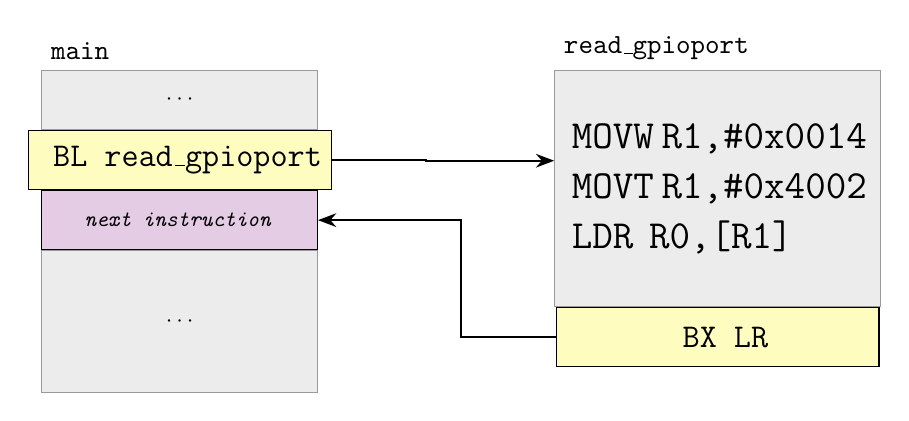
\begin{tikzpicture}[
				>=Stealth,
				font=\ttfamily\footnotesize,
				box/.style={
					draw=gray!80,
					fill=gray!15,
					minimum width=3.5cm,
					align=left
				},
				call/.style={
					draw,
					fill=yellow!25,
					minimum width=3.5cm,
					align=left
				},
				next/.style={
					draw,
					fill=violet!20,
					minimum width=3.5cm,
					align=center
				}
				]

				%------------------------------------------------
				% LEFT COLUMN (main)
				%------------------------------------------------

				\node[box, minimum height=0.75cm] (L1) {$\cdots$};

				\node[
				anchor=south west,
				font=\ttfamily\bfseries
				] at (L1.north west) {main};

				\node[
				call,
				minimum height=0.75cm,
				below=0pt of L1
				] (L2) {\hspace{2mm}\large BL read\_gpioport};

				\node[
				next,
				minimum height=0.75cm,
				below=0pt of L2
				] (L3) {\textit{next instruction}};

				\node[
				box,
				minimum height=1.8cm,
				below=0pt of L3
				] (L4) {$\cdots$};

				%------------------------------------------------
				% RIGHT COLUMN (read_gpioport)
				%------------------------------------------------

				\node[
				box,
				text width=3.9cm,
				minimum height=3.0cm,
				anchor=north west
				] (R1) at ([xshift=3cm]L1.north east)
				{
					\Large
					\begin{tabular}{@{}l@{}}
						\texttt{~MOVW R1,\#0x0014}\\
						\texttt{~MOVT R1,\#0x4002}\\
						\texttt{~LDR\ \ R0,[R1]}
					\end{tabular}
				};

				\node[
				anchor=south west,
				font=\ttfamily\bfseries
				] at (R1.north west) {read\_gpioport};

				\node[
				call,
				minimum width=4.1cm,
				minimum height=0.75cm,
				below=0pt of R1
				] (R2) {\hspace{2mm}\large BX LR};

				%------------------------------------------------
				% CALL ARROW
				%------------------------------------------------

				\draw[->,thick]
				(L2.east)
				-- ++(1.2,0)
				|- ([yshift=10pt]R1.west);

				%------------------------------------------------
				% RETURN ARROW
				%------------------------------------------------

				\draw[->,thick]
				(R2.west)
				-- ++(-1.2,0)
				|- (L3.east);

			\end{tikzpicture}}
		\end{column}
	\end{columns}

	\vspace{2mm}
	{\small\centering \alert{\texttt{BL} calls a subroutine; \texttt{BX LR} returns from it.}\par}
\end{frame}

\begin{frame}[fragile]{Returning a Value}
	\leavevmode
	{\small How does a subroutine hand a result back? By another
	convention: the return value goes in \alert{\texttt{R0}}.}

	\vspace{2mm}
	\begin{lstlisting}[style=armasm, basicstyle=\small\ttfamily]
read_gpioport
		MOVW  R1, #0x0014   ; GPIOA_IDR low half
		MOVT  R1, #0x4002   ; GPIOA_IDR high half
		LDR   R0, [R1]      ; read GPIO input register
		BX    LR            ; return, with result in R0
	\end{lstlisting}

	\vspace{2mm}
	\begin{lstlisting}[style=armasm, basicstyle=\small\ttfamily]
		BL    read_gpioport
		; R0 now contains the GPIO port value
	\end{lstlisting}

	\vspace{2mm}
	{\small \texttt{read\_gpioport} takes no arguments, yet still returns a
	value --- the two conventions are independent. The next slide shows
	\texttt{R0} used for an argument \alert{too}.}
\end{frame}

\begin{frame}[fragile]{Passing Arguments}
	\leavevmode
	{\small Now consider a function that needs information \emph{from} its
	caller:}

	\begin{lstlisting}[style=myc]
uint32_t read_bit(uint32_t port, uint32_t mask) {
    return port & mask;
}
	\end{lstlisting}

	\vspace{2mm}
	\begin{columns}[T]
		\begin{column}{.5\textwidth}
			{\small The first four 32-bit arguments travel in \texttt{R0}--\texttt{R3}:
			\begin{itemize}\itemsep1pt
				\item \texttt{R0} = \texttt{port}
				\item \texttt{R1} = \texttt{mask}
				\item \texttt{R0} = result, on return
			\end{itemize}

			\vspace{1mm}
			\texttt{R0} therefore plays two roles at different points in the
			same call: it carries a value \alert{in}, as the first argument,
			and it carries the result \alert{out}, once the function
			returns.}
		\end{column}
		\begin{column}{.46\textwidth}
			\begin{lstlisting}[style=armasm, basicstyle=\small\ttfamily]
read_bit
    AND   R0, R0, R1
    BX    LR
			\end{lstlisting}
		\end{column}
	\end{columns}

	\vspace{2mm}
	{\small \texttt{R0}--\texttt{R1} for arguments, \texttt{R0} for the return
	value --- this is not a rule invented for one function. It is a shared
	convention every function obeys. Two more leaf subroutines show it holding
	under slightly different conditions, before asking what happens once one
	subroutine calls another.}
\end{frame}

\begin{frame}[fragile]{Worked Example: A Value That Must Survive}
    \leavevmode
    {\small \texttt{read\_gpioport} and \texttt{counter} share the same shape
    --- no parameters, one result in \texttt{R0}, a leaf function --- but
    \texttt{counter} needs something \texttt{read\_gpioport} did not: a value
    still there the \alert{next} time it is called.}

    \vspace{2mm}
    \begin{columns}[T]
    \begin{column}{.46\textwidth}
        \begin{lstlisting}[style=myc, basicstyle=\normalsize\ttfamily]
int counter(void) {
    static int n = 0;
    return ++n;
}
        \end{lstlisting}
    \end{column}
    \begin{column}{.5\textwidth}
        \begin{lstlisting}[style=armasm, basicstyle=\normalsize\ttfamily]
counter
     LDR   R0, =n
     LDR   R1, [R0]
     ADDS  R1, R1, #1
     STR   R1, [R0]
     MOV   R0, R1
     BX    LR
        \end{lstlisting}
    \end{column}
    \end{columns}

    \vspace{3mm}
\begin{block}{A register cannot hold \texttt{n}} Every register's contents are gone the moment the function returns. \texttt{n} must live in \alert{memory}, at a fixed address, like any global or static variable. The register traffic here only gets that value into \texttt{R0} and back out again. \end{block}
\end{frame}

\begin{frame}[fragile]{Worked Example: \texttt{x = foo(y, z)}}
    \leavevmode
    {\small \texttt{read\_bit} returned the result of a single \texttt{AND}.
    A real function body is rarely that short:}

    \vspace{1mm}
    \begin{columns}[T]
    \begin{column}{.34\textwidth}
        \begin{lstlisting}[style=myc, basicstyle=\normalsize\ttfamily]
int foo(int a, int b) {
    return a * 2 + b;
}

x = foo(y, z);
        \end{lstlisting}
    \end{column}
    \begin{column}{.6\textwidth}
        \begin{lstlisting}[style=armasm, basicstyle=\normalsize\ttfamily]
foo
     LSLS  R0, R0, #1   ; a*2
     ADDS  R0, R0, R1   ; +b
     BX    LR
        \end{lstlisting}

        \vspace{2mm}
        \begin{lstlisting}[style=armasm, basicstyle=\normalsize\ttfamily]
; y already in R0, z in R1
     BL    foo
     MOVS  R4, R0        ; x = result
        \end{lstlisting}
    \end{column}
    \end{columns}

    \vspace{3mm}
\begin{block}{Same convention, more work inside} \texttt{a*2} is the shift-instead-of-multiply trick from Chapter~6 --- the calling convention changes nothing about how the body is optimised. \texttt{R0} still carries the argument in and the result out, exactly as \texttt{read\_bit} showed; only the number of instructions in between has grown. \end{block}
\end{frame}

\begin{frame}[fragile]{The Internals Can Change Without the Caller Knowing}
    \leavevmode
    {\small Every example so far has had exactly one implementation. Consider
    a function called exactly like any other:}

    \begin{lstlisting}[style=myc]
int popcount(uint32_t x);
...
int n = popcount(mask);
    \end{lstlisting}

    \vspace{2mm}
    {\small A straightforward version checks every bit, shifting right until
    nothing remains --- the same loop as the earlier Popcount example, now
    wrapped as a callable function:}

    \begin{lstlisting}[style=armasm, basicstyle=\small\ttfamily]
popcount
    MOV   R1, #0        ; count = 0
loop
    ANDS  R2, R0, #1    ; check bit 0
    ADD   R1, R1, R2    ; count += bit
    LSRS  R0, R0, #1    ; next bit
    BNE   loop
    MOV   R0, R1
    BX    LR
    \end{lstlisting}
\end{frame}

\begin{frame}[fragile]{A Faster \texttt{popcount}: Same Signature}
    \leavevmode
    {\small One loop iteration per \alert{bit position} --- 32 in the worst
    case. A well-known trick does better: \texttt{x \& (x - 1)} clears the
    \alert{lowest set bit}, so the loop runs once per 1 bit, not once per
    position.}

    \vspace{1mm}
    \begin{lstlisting}[style=armasm, basicstyle=\small\ttfamily]
popcount
    MOV   R1, #0        ; count = 0
    CMP   R0, #0
    BEQ   done
loop
    ADD   R1, R1, #1    ; count++
    SUBS  R2, R0, #1    ; R2 = x - 1
    ANDS  R0, R0, R2    ; x &= (x - 1)
    BNE   loop
done
    MOV   R0, R1
    BX    LR
    \end{lstlisting}

\begin{block}{Same signature, same calling sequence --- different caller cannot tell}
    Argument in \texttt{R0}, result in \texttt{R0}, \texttt{BX LR} to return
    --- identical to the first version. A function's internals can be
    rewritten and replaced, and every caller keeps working untouched.
\end{block}
\end{frame}

%===============================================================================
\section{Nested Functions}
%===============================================================================



\begin{frame}{Leaf Versus Non-Leaf Subroutines}
	\leavevmode
	\begin{columns}[T]
		\begin{column}{.42\textwidth}
			{\small
				\begin{itemize}\itemsep3pt
					\item A \alert{leaf} subroutine does not call
					another subroutine. It executes no \texttt{BL}, so
					its \texttt{LR} remains unchanged.

					\item A \alert{non-leaf} subroutine calls another
					subroutine. Its next \texttt{BL} will overwrite
					the value currently in \texttt{LR}.
			\end{itemize}}

			\vspace{2mm}
			{\small
				This gives us an important rule:

				\vspace{1mm}
				\begin{center}
					\alert{A non-leaf subroutine must save its
						\texttt{LR} before making another call.}
				\end{center}

				The stack provides a convenient place to save it.
			}
		\end{column}

		\begin{column}{.54\textwidth}
			\begin{center}
				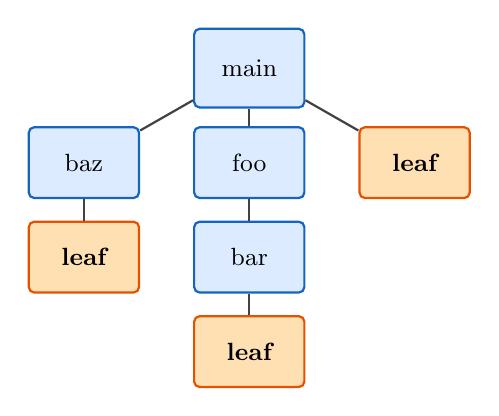
\begin{tikzpicture}[x=14mm, y=12mm,
					every node/.style={font=\scriptsize}]
					\node[blk, minimum width=14mm, minimum height=10mm]
					(main) at (1.5,3) {main};
					\node[blk, minimum width=14mm]
					(foo) at (0,2) {baz};
					\node[blk, minimum width=14mm]
					(bar) at (1.5,2) {foo};
					\node[cpublk, minimum width=14mm]
					(leaf1) at (3,2) {leaf};
					\node[cpublk, minimum width=14mm]
					(leaf2) at (0,1) {leaf};
					\node[blk, minimum width=14mm]
					(baz) at (1.5,1) {bar};
					\node[cpublk, minimum width=14mm]
					(leaf3) at (1.5,0) {leaf};

					\draw[busline] (main) -- (foo);
					\draw[busline] (main) -- (bar);
					\draw[busline] (main) -- (leaf1);
					\draw[busline] (foo) -- (leaf2);
					\draw[busline] (bar) -- (baz);
					\draw[busline] (baz) -- (leaf3);
				\end{tikzpicture}
			\end{center}

			\vspace{1mm}
			{\small\centering
				\alert{Filled} boxes are leaf subroutines.
				Plain boxes call another subroutine and therefore
				\alert{must preserve \texttt{LR}}.\par}
		\end{column}
	\end{columns}
\end{frame}

\begin{frame}[plain]{The Problem: A Second \texttt{BL} Overwrites \texttt{LR}}
	\leavevmode

	{\small
		Consider this three-level call:
		\texttt{main} calls \texttt{foo}, and \texttt{foo} calls
		\texttt{bar}.
	}

	\vspace{2mm}
	\begin{center}
		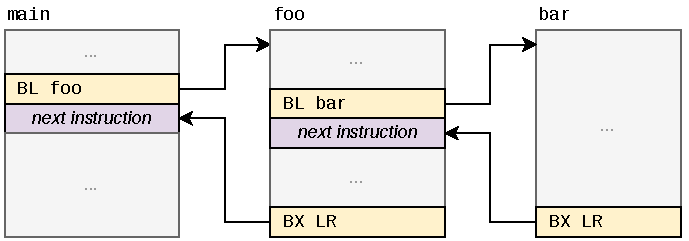
\includegraphics[]{assets/bl_foo_bar.pdf}
	\end{center}

	\vspace{3mm}
	{\small
		When \texttt{main} executes \texttt{BL foo}, the return address
		for \texttt{main} is placed in \alert{\texttt{LR}}.

		\vspace{1mm}
		But then \texttt{foo} executes \texttt{BL bar}. This places a
		new return address in the same register, \alert{overwriting the
			original address}.

		\vspace{1mm}
		Now \texttt{bar} can return to \texttt{foo}, because
		\texttt{LR} contains the correct address for that return.
		However, the original return address back to \texttt{main}
		has been lost.

		\vspace{1mm}
		\begin{center}
			\alert{One register cannot hold two return addresses.}
		\end{center}
	}
\end{frame}


\begin{frame}[fragile]{Saving the Return Address}
	\begin{columns}[T]
		\begin{column}{.6\textwidth}
			\begin{lstlisting}[style=armasm, basicstyle=\small\ttfamily]
		BL    AddNumbers

AddNumbers
		PUSH  {LR}      ; save caller's return address
		ADD   R0, R0, R1
		POP   {PC}      ; restore and return
			\end{lstlisting}

			\vspace{3mm}
			{\small
				Before making another call, a non-leaf subroutine
				can move its return address from \texttt{LR} to the
				stack:

				\begin{center}
					\texttt{PUSH \{LR\}}
				\end{center}

				This preserves the address even when a later
				\texttt{BL} overwrites \texttt{LR}.

				\vspace{1mm}
				At the end, \texttt{POP \{PC\}} restores the saved
				address directly into the program counter, returning
				execution to the caller.
			}
		\end{column}

		\begin{column}{.38\textwidth}
			\begin{block}{The key idea}
				\texttt{LR} is convenient for a single call, but it
				cannot preserve multiple return addresses.

				\vspace{2mm}
				\alert{The stack turns one temporary register into
					persistent storage for the return address.}
			\end{block}

			\vspace{2mm}
			{\small
				A leaf subroutine does not need this step: because it
				makes no further call, its \texttt{LR} remains intact
				and it can return with \texttt{BX LR}.
			}
		\end{column}
	\end{columns}
\end{frame}


\begin{frame}[plain]{The Stack Can Save More Than \texttt{LR}}
	\leavevmode

	\begin{center}
		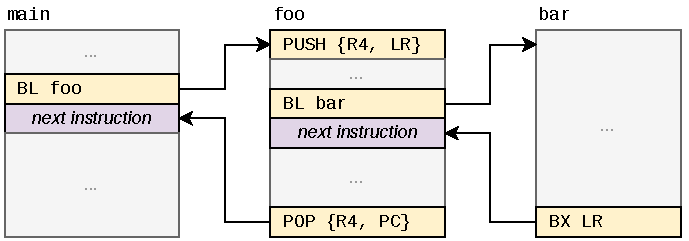
\includegraphics[]{assets/safe_bl_foo_bar.pdf}
	\end{center}

	\vspace{3mm}
	{\small
		\texttt{PUSH} can save several registers in one instruction.
		For example,
		\texttt{PUSH \{R4, LR\}} saves both \texttt{R4} and the
		return address on the stack.

		\vspace{1mm}
		When the subroutine finishes, the same registers can be restored
		with
		\texttt{POP \{R4, PC\}}.

		\vspace{1mm}
		Restoring \texttt{LR} into \texttt{PC} returns execution to the
		caller, while restoring \texttt{R4} returns it to its original
		value.
	}
\end{frame}

%-------------------------------------------------------------------------------

%\begin{frame}[plain]{2. A Second \texttt{BL} Overwrites LR}
%	\leavevmode
%
%
%	{\small
%		Now \texttt{foo} calls \texttt{bar}. The second \texttt{BL}
%		needs to put a new return address in the \alert{same LR register}.
%	}
%
%	\vspace{3mm}
%
%	\begin{center}
%		\begin{tikzpicture}[
%			x=10mm, y=9mm,
%			every node/.style={font=\scriptsize},
%			func/.style={
%				draw=black!55,
%				rounded corners=1mm,
%				minimum width=27mm,
%				minimum height=13mm,
%				align=center
%			},
%			reg/.style={
%				draw=primary,
%				fill=primary!10,
%				rounded corners=1mm,
%				minimum width=29mm,
%				minimum height=13mm,
%				align=center
%			},
%			stackcell/.style={
%				draw=black!45,
%				minimum width=25mm,
%				minimum height=8mm,
%				align=center
%			}
%			]
%
%			% Program
%			\node[func] (main) at (0,1.7)
%			{\texttt{main}\\\scriptsize caller};
%
%			\node[func] (foo) at (4.0,1.7)
%			{\texttt{foo}\\\scriptsize BL bar};
%
%			\node[func, fill=secondary!10] (bar) at (7.8,1.7)
%			{\texttt{bar}\\\scriptsize BX LR};
%
%			% Main -> foo
%			\draw[-{Stealth[length=2.2mm]}, thick, black!55]
%			(main.east) -- (foo.west);
%
%			% foo -> bar
%			\draw[-{Stealth[length=2.2mm]}, thick, secondary]
%			(foo.east) -- node[above, font=\scriptsize\bfseries]
%			{\texttt{BL bar}} (bar.west);
%
%			% LR
%			\node[reg] (lr) at (4.0,-0.3)
%			{\texttt{LR}\\[-1mm]
%				\scriptsize now: return to \texttt{foo}};
%
%			% Old value
%			\draw[-{Stealth[length=2mm]}, thick, black!45, dashed]
%			(main.south) to[bend right=18]
%			node[left, font=\tiny, text=black!55]
%			{old value:\\return to main}
%			(lr.west);
%
%			% New value
%			\draw[-{Stealth[length=2mm]}, thick, secondary]
%			(bar.south) to[bend left=18]
%			node[right, font=\tiny, text=secondary]
%			{new value:\\return to foo}
%			(lr.east);
%
%			% Stack
%			\node[lbl, font=\scriptsize\bfseries] at (8.0,-1.7)
%			{stack};
%
%			\node[stackcell, draw=black!25, dashed, text=black!45]
%			at (8.0,-2.4) {empty};
%
%			% Problem
%			\node[
%			draw=primary,
%			fill=primary!7,
%			rounded corners=1mm,
%			align=center,
%			minimum width=31mm,
%			minimum height=11mm,
%			font=\scriptsize
%			] at (3.9,-2.7)
%			{\alert{main's return address}\\\alert{has been overwritten}};
%
%		\end{tikzpicture}
%	\end{center}
%
%	\vspace{2mm}
%
%	{\small
%		The first return address is gone. When \texttt{bar} returns,
%		\texttt{LR} correctly points back to \texttt{foo}; but after that,
%		\texttt{foo} has no way to recover its original return address
%		to \texttt{main}.
%	}
%
%	\vspace{2mm}
%
%	\begin{block}{The problem}
%		\centering
%		\alert{\texttt{LR} can hold one return address, but nested calls need more than one.}
%	\end{block}
%
%\end{frame}

%-------------------------------------------------------------------------------

%\begin{frame}[plain]{3. Save LR on the Stack Before Calling Again}
%	\leavevmode
%
%
%	{\small
%		The solution is to move the first return address out of
%		\alert{\texttt{LR}} before making another call.
%		The stack provides a safe place to keep it.
%	}
%
%	\vspace{3mm}
%
%	\begin{center}
%		\begin{tikzpicture}[
%			x=10mm, y=8mm,
%			every node/.style={font=\scriptsize},
%			func/.style={
%				draw=black!55,
%				rounded corners=1mm,
%				minimum width=25mm,
%				minimum height=13mm,
%				align=center
%			},
%			reg/.style={
%				draw=primary,
%				fill=primary!10,
%				rounded corners=1mm,
%				minimum width=27mm,
%				minimum height=12mm,
%				align=center
%			},
%			stackcell/.style={
%				draw=primary,
%				fill=primary!10,
%				minimum width=31mm,
%				minimum height=9mm,
%				align=center
%			}
%			]
%
%			% Program
%			\node[func] (main) at (0,2.0)
%			{\texttt{main}\\\scriptsize BL foo};
%
%			\node[func] (foo) at (4.0,2.0)
%			{\texttt{foo}\\\scriptsize PUSH \{LR\}\\
%				\scriptsize BL bar};
%
%			\node[func, fill=secondary!10] (bar) at (8.0,2.0)
%			{\texttt{bar}\\\scriptsize BX LR};
%
%			% Calls
%			\draw[-{Stealth[length=2.2mm]}, thick, black!55]
%			(main.east) -- (foo.west);
%
%			\draw[-{Stealth[length=2.2mm]}, thick, secondary]
%			(foo.east) -- node[above, font=\scriptsize\bfseries]
%			{\texttt{BL bar}} (bar.west);
%
%			% LR
%			\node[reg] (lr) at (4.0,-0.2)
%			{\texttt{LR}\\[-1mm]
%				\scriptsize return to \texttt{foo}};
%
%			% Stack
%			\node[lbl, font=\scriptsize\bfseries] at (8.0,-0.3)
%			{stack};
%
%			\node[stackcell] (saved) at (8.0,-1.0)
%			{\texttt{LR} saved\\\scriptsize return to main};
%
%			\node[stackcell, draw=black!25, dashed, text=black!45]
%			at (8.0,-1.9) {free};
%
%			% LR -> stack
%			\draw[-{Stealth[length=2.2mm]}, thick, primary]
%			(lr.east) to[bend left=18]
%			node[above, font=\tiny, text=primary]
%			{\texttt{PUSH \{LR\}}}
%			(saved.west);
%
%			% Stack pointer
%			\draw[flow, thick]
%			(saved.south west) ++(-0.2,0)
%			-- ++(-0.8,0)
%			node[left, font=\tiny] {\texttt{SP}};
%
%			% New LR
%			\node[
%			draw=secondary,
%			fill=secondary!10,
%			rounded corners=1mm,
%			minimum width=27mm,
%			minimum height=11mm,
%			align=center,
%			font=\scriptsize
%			] at (4.0,-2.8)
%			{\texttt{LR}\\\scriptsize return to \texttt{bar}};
%
%			\draw[-{Stealth[length=2mm]}, thick, secondary]
%			(bar.south) to[bend left=18]
%			node[right, font=\tiny, text=secondary]
%			{new return address}
%			(4.0,-2.25);
%
%		\end{tikzpicture}
%	\end{center}
%
%	\vspace{2mm}
%
%	{\small
%		Now the two return addresses have different homes:
%		the current one remains in \texttt{LR}, while the older one is
%		safely stored on the stack. When \texttt{bar} returns, \texttt{foo}
%		can restore the saved address with \texttt{POP \{PC\}}.
%	}
%
%	\vspace{2mm}
%
%	\begin{block}{The complete pattern}
%		\centering
%		\texttt{PUSH \{LR\}} \quad $\rightarrow$ \quad
%		\texttt{BL} \quad $\rightarrow$ \quad
%		\texttt{POP \{PC\}}
%
%		\vspace{1mm}
%		\scriptsize
%		Save the old return address $\rightarrow$ make the nested call
%		$\rightarrow$ restore and return
%	\end{block}
%
%
%\end{frame}


\begin{frame}{Why a Call Needs More Than Registers}
    \leavevmode
    {\small The examples so far passed arguments in \texttt{R0}/\texttt{R1} and
    returned a result in \texttt{R0}, by convention. The nested-call problem
    just solved --- save \texttt{LR} before a second \texttt{BL} --- raises the
    same question one level up: \alert{which} registers are safe to overwrite,
    and which must a callee restore?}

    \vspace{2mm}
    {\small Every function you write, and every library function you call,
    needs the \emph{same} answer to that question --- otherwise C code and
    hand-written assembly could never call each other safely. That shared
    answer is a formal convention: the \alert{AAPCS}.}
\end{frame}

%===============================================================================
\section{The AAPCS}
%===============================================================================

%===============================================================================

\begin{frame}{How Do Two Functions Agree on Anything?}
    \leavevmode
{\small
	Your C code and a library compiled years ago must agree on where
	arguments go, where results return, and who preserves what ---
	with no run-time negotiation.}

    \vspace{3mm}
    \begin{center}
    \begin{tikzpicture}[x=13mm, y=10mm]
        \node[blk, minimum width=20mm, minimum height=20mm] (caller) at (0,0) {caller};
        \node[cpublk, minimum width=20mm, minimum height=20mm] (callee) at (5,0) {callee};

        \draw[flow] ([yshift=5mm]caller.east) -- node[lbl, above, font=\scriptsize]
             {R0 = argument 1} ([yshift=5mm]callee.west);
        \draw[flow] (caller.east) -- node[lbl, above, font=\scriptsize]
             {R1 = argument 2} (callee.west);
        \draw[flow, draw=primary] ([yshift=-6mm]callee.west) -- node[lbl, below, text=primary, font=\scriptsize]
             {R0 = return value} ([yshift=-6mm]caller.east);
    \end{tikzpicture}
    \end{center}

\vspace{2mm} \textbf{\small Procedure Call Standard for the ARM Architecture (AAPCS)} \vspace{1mm} \begin{block}{The AAPCS is that agreement} It defines where arguments and return values go and which registers a function must preserve. This lets C and assembly functions call each other safely. \end{block}
\end{frame}

\begin{frame}{The AAPCS}{The contract between functions}
    \begin{center}
    {\small
    \striped
    \begin{tabular}{@{}l R{.62\textwidth}@{}}
\toprule
\textbf{Registers} & \textbf{Rule} \\
\midrule
\texttt{R0}--\texttt{R3}
& Arguments 1--4; \texttt{R0} also carries the return value. \alert{Caller-saved}: the callee may overwrite them. \\[1mm]
\texttt{R4}--\texttt{R11}
& \phantom{}\alert{Callee-saved}: the callee must restore any it uses. \\
\texttt{R12}
& Scratch register. \\
\texttt{R13}--\texttt{R15}
& SP, LR, PC. \\
\bottomrule
    \end{tabular}}
    \end{center}

    \vspace{3mm}
    {\small Arguments beyond the fourth go on the \alert{stack} ---
    the same mechanism just used to save \texttt{LR}.}
\end{frame}

\begin{frame}[fragile]{Do No Damage: Callee-Saved Registers}
	\leavevmode
	{\small
    			A function may use \texttt{R4}--\texttt{R11}, but it must restore
    			them before returning. The pattern is the same as saving
    			\texttt{LR}: \alert{save, use, restore}.}

    \vspace{2mm}
    \begin{lstlisting}[style=armasm, basicstyle=\small\ttfamily]
foo  PUSH {R4, R5}    ; save registers this function will use
     MOV  R4, #0
     MOV  R5, #0xAB
     ADD  R4, R4, R5
     ...
     POP  {R4, R5}    ; restore their original values
     BX   LR
    \end{lstlisting}

    \vspace{2mm}
\begin{block}{Why this matters} The caller can continue using \texttt{R4} and \texttt{R5} after \texttt{foo} returns, knowing their values are unchanged. No special agreement is needed at each call site. \end{block}
\end{frame}


\begin{frame}{Summary}
    \leavevmode
    {\small The whole chapter is one causal chain:}

    \vspace{2mm}
    \begin{center}
    {\small
    C condition $\rightarrow$ \texttt{CMP}/\texttt{S} suffix
    $\rightarrow$ APSR flags $\rightarrow$ conditional branch
    $\rightarrow$ \texttt{if}/loop
    \\[1mm]
    \texttt{BL} $\rightarrow$ \texttt{LR} $\rightarrow$ nested call
    overwrites \texttt{LR} $\rightarrow$ \texttt{PUSH}/\texttt{POP}
    $\rightarrow$ stack
    \\[1mm]
    stack $\rightarrow$ \textbf{AAPCS} $\rightarrow$ functions can
    safely call each other}
    \end{center}

    \vspace{3mm}
    \begin{itemize}\itemsep1pt
        \item \textbf{Signed} codes (\texttt{GE}, \texttt{LT}) for signed
              data; \textbf{unsigned} codes (\texttt{HS}, \texttt{LO}) for
              unsigned data. Every branch tests the \emph{opposite} of the
              C condition.
        \item \textbf{Counting down with \texttt{SUBS}} is cheaper than
              counting up with \texttt{CMP} --- one instruction, two jobs.
        \item A \textbf{non-leaf} subroutine must save \texttt{LR} on the
              \textbf{full descending} stack before its own \texttt{BL}
              can overwrite it. A \textbf{leaf} subroutine does not.
        \item The \textbf{AAPCS} fixes how arguments are passed and which
              registers a function must preserve.
    \end{itemize}

    \vspace{2mm}
    \begin{block}{Next: Chapter 8 --- General Purpose Input Output}
        The book stops being theory here. Next, a physical pin actually
        changes voltage.
    \end{block}
\end{frame}


%===============================================================================
\section{Design Challenge}
%===============================================================================

\begin{frame}{Design Challenge}{To be worked on paper, before any code}
    \leavevmode
    \begin{block}{The brief}
        A safety interlock must poll four sensors and respond within 500~\textmu s of any one of them going out of range, on a 16~MHz processor.
    \end{block}

    \vspace{2mm}
    {\small Design the control flow before writing code: decide whether the four checks should be a sequence of \texttt{if} statements, a loop over an array, or a table of function pointers, and justify the choice in terms of the instructions each becomes. Work out the worst-case instruction budget available. Then state which of the three designs you could check by reading its disassembly, and what you would look for.}
\end{frame}

\begin{frame}[plain]
    \begin{center}
        \vfill
        {\usebeamerfont{title}\color{primary}\Huge Questions?}
        \vfill
        {\small\color{Gray} \emph{Introduction to ARM Cortex-M Microprocessors} --- Chapter 7}
        \vfill
    \end{center}
\end{frame}

\end{document}
